\section{Feature-First Block Model}

In this section we propose a novel generative model for labelled networks. We call this the feature-first block model (FFBM),
illustrated in Figure~\ref{fig:ffbm}.

Let $N$ denote the number of vertices, $B$ the number of blocks
and ${\cal X}$ the set of values each feature can take.
We define the vector $x_i \in \mathcal{X}^D$ as the feature vector for vertex $i$, 
where $D$ is the number of features associated with each vertex.
For example, in the datasets we analyse, we deal with binary feature flags
(denoting the presence/absence of each feature),
so $\mathcal{X} = \{0, 1\}$. We write $X$ for the $N\times D$ {\em feature matrix} containing
the feature vectors $\{x_i\}_{i=1}^{N}$ 
as its rows.

For the FFBM, we start with the feature matrix $X$ and generate a random
vector of block memberships $b \in [B]^N$. For each vertex $i$, the
block membership $b_i\in[B]$ is generated based on the feature
vector $x_i$, independently between vertices. The conditional
distribution of $b_i$ given $x_i$ also depends on a collection
of weight vectors $\theta=\{w_k\}_{k=1}^B$, where each
$w_k$ has dimension $D$. We will later find it convenient
to write $\theta$ as a $B \times D$ matrix of weights $W$. Specifically, 
the distribution of $b$ given $X$ and $\theta$ is,
%
\begin{equation}
	p(b| X, \theta) = \prod_{i \in [N]} p(b_i | x_i, \theta) = \prod_{i \in [N]} \phi_{b_i} (x_i; \theta)
	= \prod_{i \in [N]} \frac{\exp\left(w_{b_i}^T x_i\right)}{\sum_{k \in [B]} \exp \left( w_k^T x_i\right)}.
\end{equation}
%
Note that $\phi_{b_i}$ has the form of a softmax activation function.
More complex models based on different choices for the distributions
$\phi_{b_i}$ above are also possible, but then deriving meaning from 
the inferred parameter distributions is more difficult. 
%
\begin{figure}[!ht]
	\centering
%	\begin{tikzpicture}[
%		roundnode/.style={circle, draw=black, minimum size=7mm},
%		squarednode/.style={rectangle, draw=black, minimum size=7mm}
%		]
%		% nodes
%		\node[roundnode] (X) at (0, 0) {$X$};
%		\node[squarednode] (b) at (3, 0) {$b$};
%		\node[roundnode] (A) at (6, 0) {$A$};
%		
%		% arrows
%		\draw[->] (X.east) -- node[above] {$\theta$} (b.west);
%		\draw[->] (b.east) -- node[above] {$\psi$}(A.west);
%	\end{tikzpicture}
	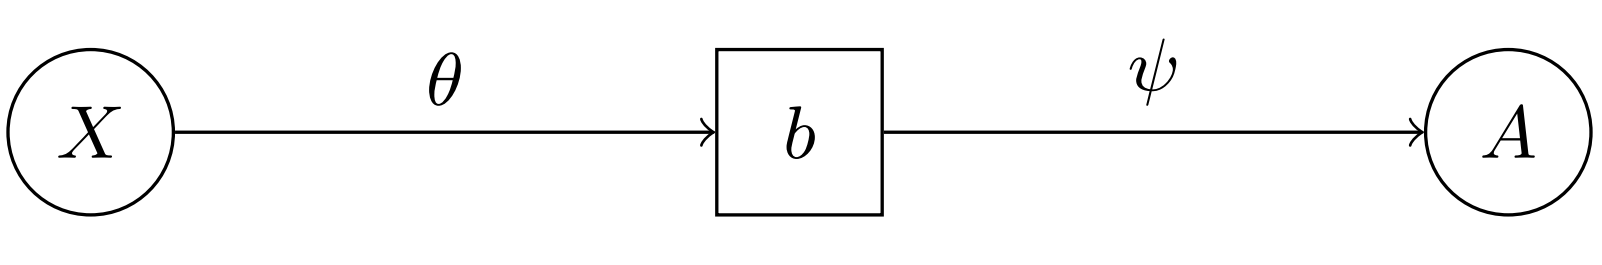
\includegraphics[width=0.8\textwidth]{img/ffbm.png}
	\caption{The Feature-First Block Model (FFBM)}
	\label{fig:ffbm}
\end{figure}

Once the block memberships $b$ have been generated, we then draw the 
graph $A$ from the microcanonical DC-SBM with additional parameters 
$\psi = \{\psi_e, \psi_k\}$:
%
\begin{equation}
	A \sim \textrm{DC-SBM}_{\textrm{MC}} (b, \psi_e, \psi_k).
	\label{eqn:A-generation}
\end{equation}
